Производить локальное измельчение сетки можно различными путями, основываясь на геометрии рассматриваемой области $G\subset\mathbb{R}^p$, геометрии множества особых точек уравнения, принятой неравномерной/криволинейной сетки.
Подход, который используется в работе, основан на декартовых прямоугольных сетках.
Такой выбор является оптимальным с точки зрения компьютерный вычислений~--- данные легче и удобнее всего хранятся и обрабатываются в областях прямоугольной формы, в то время как неструктурированные локальные измельчения приводят к нерегулярному доступу к памяти компьютера и, тем самым, замедлением счёта.
Сущность такого подхода можно описать следующим образом: исходная прямоугольная область
$
    G = \prod_{k = 1}^{p} [0, L_p]
$
дискретизуется равномерной сеткой.
Далее в соответствии с некоторыми критериями, выделяются подобласти, в которых содержатся особенности.
Эти подобласти покрываются прямоугольными областями, которые в свою очередь дискретизуются более мелкой сеткой.
Такой процесс продолжается до тех пор, пока нужные зоны \glqq не покроются достаточно хорошо \grqq, настолько, чтобы численное решение в этих областях достигала заданной точности.
После выбора такой сетки производится численное интегрирование нескольких временных шагов.
После такого обновления решения, его особые точки могут сместиться, соответственно, придётся перестраивать сетку под особенности.
Данные переинтерполируются со старой сетки на новую, перестроенную, и процесс продолжается снова.

\begin{wrapfigure}{r}{0.5\textwidth}
    \begin{center}
        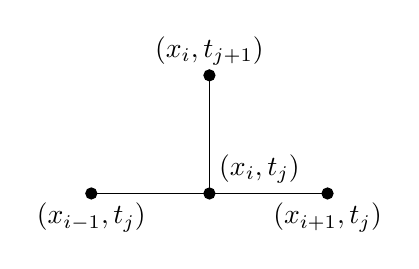
\begin{tikzpicture}
            \filldraw[black] (0, 0) circle(2pt) node[anchor=south west] {$(x_i, t_j)$};
            \draw (-1.5, 0) node[anchor=north] {$(x_{i - 1}, t_j)$} -- (1.5, 0) node[anchor=north] {$(x_{i + 1}, t_j)$};
            \filldraw[black] (-1.5, 0) circle(2pt);
            \filldraw[black] (1.5, 0) circle(2pt);
            \filldraw[black] (0, 1.5) circle(2pt);
            \draw (0, 0) -- (0, 1.5) node[anchor=south]{$(x_i, t_{j + 1})$};
        \end{tikzpicture}
    \end{center}
\end{wrapfigure}
Основная теория черпалась из работ \cite{berger1982adaptive, berger1989local, deiterding2011block}.
Однако стоит отметить следующие обстоятельства.
Во-первых, в этих статьях исследовался подход локально-адаптивных сеток применительно к уравнениям гиперболического типа.
Это позволяло использовать явную вычислительную схему, в то время как для параболических систем это ведёт к определённым условиям на выбор временного и пространственного шага.
Во-вторых, использовался так называемый клеточный подход, в котором область $G$ представлялась в виде ячеек (cells) прямоугольной формы, в цетре которых хранилось среднее значение решения (то есть использовался проекционный оператор вида $P_h = \frac{1}{\mu(C)} \int_{C} u(x)\, dx$), а также на граничах ячейки хранилась информация о потоках (поток физ. величин, входящих в уравнение) $\vec f = \vec f(u)$.
